\documentclass{jdmdh}
\usepackage[utf8]{inputenc}
\usepackage{array}
\usepackage{pgfplots}

\title{Evaluating Deep Learning Methods for Tokenization of Space-less texts in Old French and Latin}
\author[1]{Thibault Clérice}
\affil[1]{École nationale des Chartes, France} 
\affil[2]{Université Lyon 3, France} 

\corrauthor{Thibault Clérice}{thibault.clerice@chartes.psl.eu}


\begin{document}

\maketitle

\abstract{Tokenization of modern and old Western European languages seems to be fairly simple as it stands on the presence mostly of markers such as spaces and punctuation. Although, when dealing with old sources like manuscript written in \textit{scripta continua}, (1) such markers are mostly absent, (2) spelling variation and rich morphology makes dictionary based approaches difficult. We show that applying convolutional encoding to characters followed by linear categorization to word-boundary or in-word-sequence can be used to tokenize such inputs. Additionally, we release a software with a rather simple interface for tokenizing one's corpus.}

\keywords{convolutional network; scripta continua; tokenization; Latin; Old French; word segmentation}

\section{Introduction}

% To Read : Stutzmann article.

Tokenization of space-less strings is a task that is specifically difficult for computer when compared to "whathumancando". \textit{Scripta continua} is a writing phenomenon where words would not be separated by spaces and it appears to have disappeared around the 8th century (see \citet{zanna1998lecture}). Although, spacing can be somewhat erratic in later centuries (\textit{cf.} Figure \ref{fig:4lines}). In the context of text mining of HTR or OCR output, lemmatization and tokenization of medieval western languages can be a pre-processing step for further research to sustain analyses such as authorship attribution \textbf{CITE JBCAMPS ?}.

\begin{figure}
  \centering
  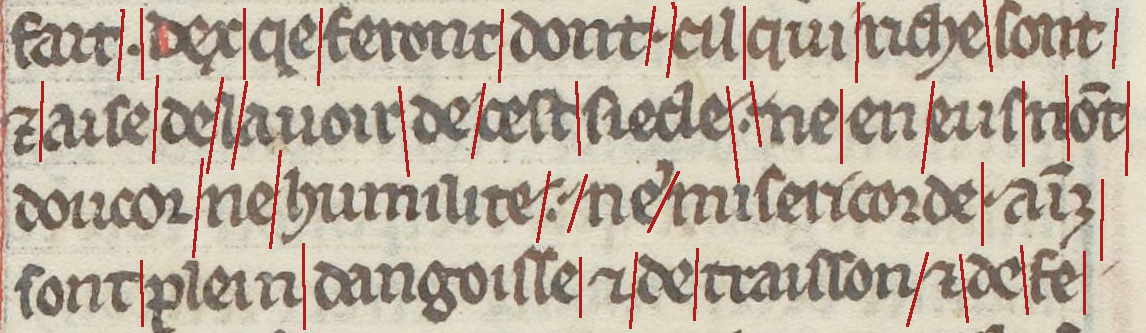
\includegraphics[width=\linewidth]{4-lines-p0215.png}

  \caption{ 4 lines from fol.103rb Manuscript fr. 412, Bibliothèque nationale de France.  Red lines indicate word boundaries}
  \label{fig:4lines}
\end{figure}

We must stress in this study that the difficulty that we face is different for \textit{scripta continua} than the ones researchers face languages such as Chinese for which an already impressive amount of work has been done as it. Indeed, Chinese word segmentation has lately been driven by deep learning methods, specifically ones based on \textit{sequence to sequence translations}: \citet{chen2015long} defines a process based on LSTM model, while \citet{yu2019learning} uses BiDirectional GRU and CRF. Actually, meanwhile redacting this article and producing the code-base, \citet{huang2019realistic} took the same approach of encoding to linear classification to both word boundary (WB) and word content (WC) for Chinese word segmentation.

\section{Description and evaluation}

\subsection{Architecture}

\subsubsection{Encoding of input and decoding}

The model is based on traditional text input encoding where each character is transcoded to an index. Output of the model is a mask that needs to be applied to the input: in the mask, characters are classified either as word boundary or word content. 

\begin{table}[]
\centering
\begin{tabular}{@{}ll@{}}
\hline
                       & \textbf{Sample}           \\  \hline
\textbf{Input  String} & \texttt{Ladamehaitees'enparti}     \\
\textbf{Mask   String} & \texttt{xSxxxSxxxxxSxxxSxxxxS}     \\
\textbf{Output String} & \texttt{La dame haitee s'en parti} \\ \hline
\end{tabular}
  \caption{Input, mask and human-readable output generated by the model. x are WC and S are WB}
  \label{lst:input_output_example}
\end{table}

For evaluation purposes, and to reduce the number of input classes, we propose both a lower-case normalization and a "reduction to the ASCII character set" feature (fr. \ref{fig:normalization}). On this point, a lot of issues were found with transliteration of MUFI characters that were part of the original datasets, as they are badly interpreted by the \texttt{unidecode} python package. Indeed, \texttt{unidecode} will simply remove characters it does not understand. An addendum to said package that would transcribe ligatures, abbreviations, etc. would probably be a good feature.

% Need a better system that this/
\begin{figure}
  \centering
  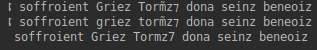
\includegraphics[width=\linewidth]{inputs.png}
  \caption{ Different possibilities of pre-processing. In the last, the first character (LATIN ABBREVIATION SIGN SMALL ET WITH STROKE) is lost by \texttt{unidecode}}
  \label{fig:normalization}
\end{figure}

\subsubsection{Model}

Each model we have used is composed of an Encoder, generally built around an embedding layer, and the same Linear Classifier. The encoders tested are:

\begin{itemize}
  \item LSTM encoder with hidden cell
  \item Convolutional (CNN) encoder with position embeddings 
  \item Convolutional (CNN) encoder without position embeddings % Currently not really because it's part of the network, but it should be for the release of the article
\end{itemize}

\subsection{Evaluation}

\subsubsection{Datasets}

Datasets are transcription from manuscripts with unresolved abbreviation coming from different projects

\begin{itemize}
    \item \textbf{Old French} based on \citet{8269990}, \citet{pinche:hal-01628533}, \citet{jean_baptiste_camps_2019_2630574}, \citet{bfmmss}, and transcription from the TNAH master at the École Nationale des Chartes.
    \begin{itemize}
        \item 193,734 training examples;
        \item 23,581 validation examples;
        \item 25,512 test examples
    \end{itemize}
\end{itemize}

\subsubsection{Results}


\begin{figure}[h!]
  \begin{center}
    \begin{tikzpicture}
      \begin{axis}[
          width=\linewidth, % Scale the plot to \linewidth
          grid=major, 
          grid style={dashed,gray!30},
          xlabel=Epoch, % Set the labels
          ylabel=Accuracy,
          legend style={at={(0.5,-0.2)},anchor=north},
          x tick label style={rotate=90,anchor=east}
        ]
        \addplot table[x=Epoch,y=CNN Train,col sep=comma] {accuracies.csv}; 
        \addplot table[x=Epoch,y=CNN No Pos,col sep=comma] {accuracies.csv}; 
        \addplot table[x=Epoch,y=CNN lower,col sep=comma] {accuracies.csv}; 
        \addplot table[x=Epoch,y=CNN norm,col sep=comma] {accuracies.csv}; 
        \legend{CNN Train,CNN without Position embedding, CNN with lowercase transform, CNN with ASCIIification}
      \end{axis}
    \end{tikzpicture}
    \caption{Training Accuracy over 50 epochs}
  \label{fig:accuracy}
  \end{center}
\end{figure}

% Include evaluation on test sets

\subsubsection{Example of outputs}

The following input was not seen during training, dev or test, and is part of a different corpus :

\begin{itemize} 
    \item \texttt{Truth :} Aies joie et leesce en ton cuer car tu auras une fille qui aura .i. fil qui sera de molt grant merite devant Dieu et de grant los entre les homes.
    \item \texttt{Input :} Aiesjoieetleesceentoncuercartuaurasunefillequiaura.i.filquiserademoltgrantmeritedevantDieuetdegrantlosentreleshomes.
    \item \texttt{CNN :} Aiesjoie et leesce en ton cuer car tu auras une fille qui aura . i . fil qui sera de molt grant merite devant Dieu et de grant los entre les homes .
    \item \texttt{CNN lower:} Aies joie et leesce en ton cuer car tu auras une fille qui aura . i . fil qui sera de molt grant merite devant Dieu et de grant los entre les homes .
    \item \texttt{CNN without position:} Aiesjoie et leesce en ton cuer car tu auras une fille qui aura . i . fil qui sera de molt grant merite devant Dieu et de grant los entre les homes .
    \item \texttt{CNN Normalize:} Aies joie et leesce en ton cuer car tu auras une fille qui aura . i . fil qui sera de molt grant merite devant Dieu et de grant los entre les homes .
\end{itemize}



\subsection{Discussion}

We believe that, aside from a graphical challenge, word segmentation in OCR from manuscripts can actually be treated from a text point of view

% "The purpose of the discussion is to interpret and describe the significance of your findings in light of what was already known about the research problem being investigated and to explain any new understanding or insights that emerged as a result of your study of the problem. The discussion will always connect to the introduction by way of the research questions or hypotheses you posed and the literature you reviewed, but the discussion does not simply repeat or rearrange the first parts of your paper; the discussion clearly explain how your study advanced the reader's understanding of the research problem from where you left them at the end of your review of prior research."

\subsection{Conclusion}

While 
% The conclusion is intended to help the reader understand why your research should matter to them after they have finished reading the paper. A conclusion is not merely a summary of the main topics covered or a re-statement of your research problem, but a synthesis of key points and, if applicable, where you recommend new areas for future research. For most college-level research papers, one or two well-developed paragraphs is sufficient for a conclusion, although in some cases, three or more paragraphs may be required.

\subsection{Acknowledgement}

Boudams has been made possible by two open-source repositories from which I learned and copied bits of implementation of certain modules and without which none of this paper would have been possible: \citet{enrique_manjavacas_2019_2654987} and \citet{bentrevett}. This tool was originally intended for post-processing OCR for the presentation \citet{pinchecampsclerice} at DH2019 in Utrecht.



\bibliographystyle{plainnat}
\bibliography{article}

\appendix\footnotesize

\section{Annex 1}
Pellentesque dignissim ultrices fringilla. Vivamus eu luctus ante, vel bibendum magna. Curabitur elit purus, tincidunt non dui
vitae, elementum bibendum neque. Curabitur ullamcorper sit amet justo at hendrerit. Fusce ut arcu imperdiet nibh mollis
tempus a aliquet tellus. Quisque pharetra cursus nisi, vel lobortis ante consectetur et. Vivamus sed congue neque. Proin
pellentesque risus nec dui consequat rutrum. Vestibulum nunc diam, placerat quis auctor vel, faucibus non justo. Etiam
dictum purus neque. Phasellus imperdiet mauris ligula, eu laoreet nisi elementum ut. Sed sed porta massa. Aenean faucibus
risus ultrices ornare porta. Quisque faucibus ante a tincidunt vestibulum. Lorem ipsum dolor sit amet, consectetur adipiscing
elit.


\section{Annex 2}
Cras tristique vel nisi at aliquet. Proin egestas erat sit amet velit lobortis imperdiet. Integer et arcu sapien. Etiam id blandit
sapien. Nam tempus lacus ac massa semper, vel laoreet turpis rutrum. Mauris eget nibh vitae justo porta imperdiet sed vel
ligula. In imperdiet, augue vel condimentum convallis, neque augue imperdiet neque, eget dapibus nunc mauris ultricies
tortor. Nam eget nunc egestas, blandit lectus non, aliquam nunc. Cras sed quam vitae arcu ornare lobortis. Ut ut lacus
hendrerit, convallis orci sit amet, commodo nunc. Pellentesque eget tincidunt tortor. Nunc ornare molestie mauris id vehicula.
Suspendisse pharetra tortor metus, sit amet fermentum tellus vehicula ut.


\end{document}